\chapter{Verificarea}


\section{Rularea inițială, fără \texttt{Eva}}

\indent\indent Recomandarea generală pentru utilizarea \texttt{frama-c}, dar și în cazul particular
al acestui proiect este să se ruleze programul din linia de comandă pe toate
sursele C ale programului, fără plugin-uri în primă fază, pentru a găsi eventualele
erori grosolane. Opțional, se poate salva rezultatul și deschide apoi în GUI sau se poate salva
într-un fișier text:

\begin{lstlisting}[language=sh,caption={\emph{Verificarea inițială a proiectului}},xleftmargin=.21\textwidth]
  # rezultate stdout:
  $ frama-c *.c
  # rezultate log
  $ frama-c *.c > log ; cat log | less
  # rezultate salvate, apoi GUI
  $ frama-c *.c -save firstrun.sav
  $ frama-c-gui -load firstrun.sav
\end{lstlisting}

În acest caz, se vor raporta:
\begin{lstlisting}[language=sh,caption={\emph{Rezultatele verificării inițiale}}]
  [kernel] Parsing monocypher.c (with preprocessing)
  [kernel] Parsing more_speed.c (with preprocessing)
  [kernel] more_speed.c:15: 
  syntax error:
  , before or at token: fe_sq
  13    
  14    // Specialised squaring function, faster than general multiplication.
  15    sv fe_sq(fe h, const fe f)
  ^^^^^^^^^^^^^^^^^^^^^^^^^^
  16    {
  17        i32 f0 = f[0]; i32 f1 = f[1]; i32 f2 = f[2]; i32 f3 = f[3]; i32 f4 = f[4];
  [kernel] Frama-C aborted: invalid user input.
\end{lstlisting}

Mai multe informații pot fi extrase din acest prim rezultat:
\begin{itemize}
\item funcția \texttt{sv fe\_sq}, care a raportat eroare, poate fi ignorată, deoarece
  nu face parte neapărat din program. Observăm că acel cod se găsește în \texttt{more\_speed.c}, care,
  conform documentației, este un fișier opțional pentru optimizare. Deocamdată, ne concentrăm
  pe codul principal;
\item Verificarea s-a terminat cu eroare, dar nu din cauzele de mai sus. Examinînd
  fișierul \texttt{makefile}, constatăm că programul se compilează cu opțiuni suplimentare,
  în acest caz, cu opțiunea de preprocesor \texttt{-DED25519\_SHA512}.
\end{itemize}

Reîncercăm și specificăm și ca verificarea să se concentreze codul principal:
\begin{lstlisting}[language=sh,caption={\emph{Verificarea inițială, corectată}}]
  $ frama-c test.c sha512.c monocypher.c \
    -cpp-extra-args="-DED25519_SHA512" -save parsed.sav
\end{lstlisting}

Execuția nu mai raportează eroare acum și într-adevăr, putem încărca în GUI rezultatul și observăm
că avem doar o mică eroare nesemnificativă într-o funcție \texttt{printf}.
\begin{figure}[!htbp]
  \centering
    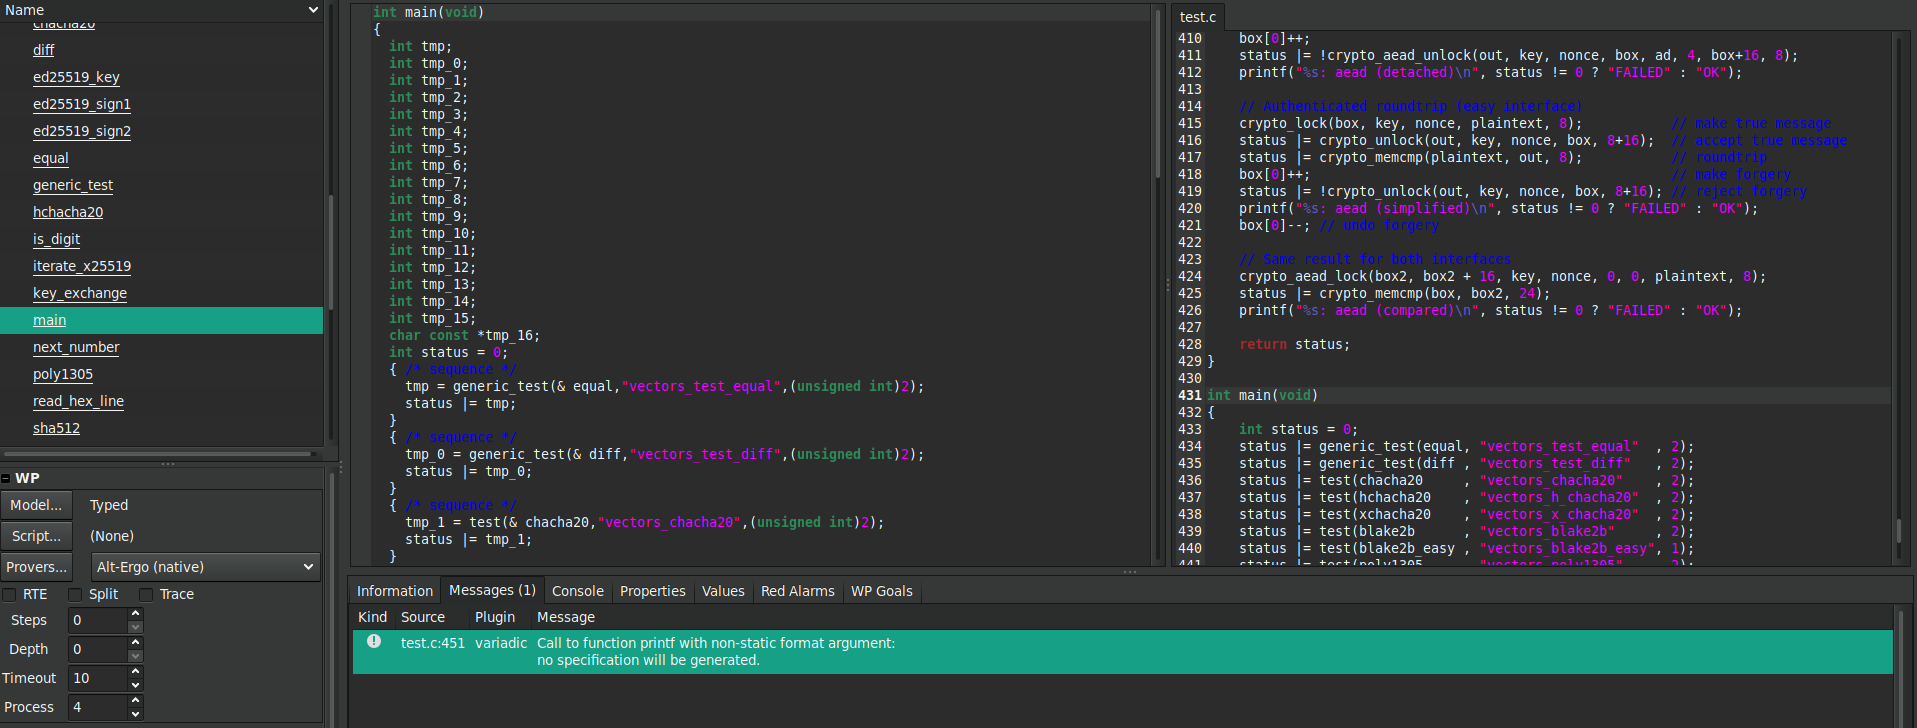
\includegraphics[width=1\textwidth]{img/framagui1.png}
    \caption{Încărcarea în GUI a rezultatelor inițiale}
\end{figure}

Concluzia acestui pas este că erorile care au mai rămas, dacă este cazul, nu sînt
majore ca să împiedice compilarea programului. El poate funcționa pe mai multe cazuri,
iar posibilele erori vor fi specifice unor cazuri anume de analiză. Trecem, atunci,
la analiza specifică folosind \texttt{Eva}.


%%%%%%%%%%%%%%%%%%%%%%%%%%%%%%%%%%%%%%%%%%%%%%%%%%%%%%%%%%%%%%%%%%%%%%
\section{Verificarea cu \texttt{Eva}}

\indent\indent Apelul la \texttt{Eva} se face cu opțiunea \texttt{-val}, deoarece programul
a evoluat din varianta \texttt{Value Analysis}.

Rularea inițială face uz doar de cîteva funcții standard, care face ca verificarea
să fie mai rapidă. Încărcăm varianta salvată din rularea standard și specificăm ca
verificarea să adauge funcții de verificare \texttt{Eva}:
\begin{lstlisting}[language=sh,caption={\emph{Verificarea inițială cu} \texttt{Eva}}]
  $ frama-c -load parsed.sav -val-builtins-auto -val -save value.sav
\end{lstlisting}

Rularea acum durează mai mult și se raportează multe alarme (posibil false),
din cauza multor operații numerice folosite în program.

De fapt, rularea de mai sus poate fi optimizată cu două opțiuni specifice:
\begin{itemize}
\item \texttt{-no-val-show-progress}, care elimină mesajele afișate cînd se intră
  într-o nouă funcție (opțiune utilă cînd sursa are multe funcții mici, ca în acest
  caz);
\item \texttt{-memexec-all}, care păstrează o parte a rezultatelor calculate
  într-un cache din memorie, pentru a nu reface toate calculele.
\end{itemize}

Așadar, rulăm cu varianta optimizată și salvăm rezultatele atît într-un binar
pentru analiză ulterioară în GUI, cît și într-un \texttt{log}.
\begin{lstlisting}[language=sh,caption={\emph{Verificarea optimizată cu Eva}}]
  $ frama-c -load parsed.sav -val -val-builtins-auto \
            -no-val-show-progress -memexec-all -save value.sav > log
\end{lstlisting}

\newpage

O selecție a liniilor din \texttt{log} afișează:
\begin{lstlisting}[language=sh,caption={\emph{Fragment din rezultatele verificării inițiale cu Eva}}]
[value] Analyzing a complete application starting at main
[value] Computing initial state
[value] Initial state computed
[value:initial-state] Values of globals at initialization
  __fc_errno in [--..--]
  __fc_stderr in {{ NULL ; &S___fc_stderr[0] }}
  __fc_stdin in {{ NULL ; &S___fc_stdin[0] }}
  __fc_stdout in {{ NULL ; &S___fc_stdout[0] }}
  __fc_fopen[0..15] in {0}
  __fc_p_fopen in {{ &__fc_fopen[0] }}
  __fc_heap_status in [--..--]
  __fc_random_counter in [--..--]
  __fc_rand_max in {32767}
  __fc_mblen_state in [--..--]
  __fc_mbtowc_state in [--..--]
  __fc_wctomb_state in [--..--]
  __fc_strtok_ptr in {0}
  K[0] in {4794697086780616226}
   [1] in {8158064640168781261}
   [2] in {13096744586834688815}
   ...
  blake2b_compress_sigma[0][0] in {0}
                        [0][1] in {1}
                        [0][2] in {2}
   ...
[value:alarm] test.c:126: Warning: 
  out of bounds write. assert \valid(v->buf + v->size);
[value:alarm] test.c:121: Warning: 
  function memcpy: precondition 'valid_src' got status unknown.
[value:alarm] monocypher.c:839: Warning: 
  signed overflow. assert g3 * 19 leq 2147483647;
[kernel] monocypher.c:494: 
  more than 200(253) locations to update in array. Approximating.
\end{lstlisting}

Cîteva comentarii esențiale pe marginea acestui raport:
\begin{itemize}
\item primele 3 linii arată că se folosește plugin-ul \texttt{Eva} (\texttt{[value]}) și
  se calculează starea inițială a programului, dată de valorile inițiale ale variabilelor;
\item liniile 5-25 arată aceste valori inițiale pentru variabilele din program;
\item alarma din linia 26 arată că o valoare a depășit valorile permise și se sugerează
  o adnotare de tipul \texttt{assert} în cod, în \texttt{test.c:126} pentru a elimina
  acest risc;
\item similar și în cazul funcției \texttt{memcpy} din \texttt{test.c:121}, caz în care
  se sugerează o adnotare de tipul unei precondiții;
\item alarma din liniile 30-31 arată că nu calcul este posibil să depășească limitele
  tipului de dată și se sugerează o adnotare de tipul \texttt{assert};
\item mesajul din liniile 32-33 este la nivelul \texttt{kernel}, adicâ nivelul fundamental
  al verificării și arată că plugin-ul (\texttt{Eva}, în acest caz) are prea multe valori
  de verificat și actualizat, deci va folosi aproximații care pot da erori (pe lîngă cele
  inerente interpretării abstracte).
\end{itemize}

Mai remarcăm de asemenea că toate aceste mesaje sînt \emph{alarme}, deci nu se știe
cu certitudine dacă sînt erori, putînd fi datorate metodei teoretice propriu-zise.
Într-adevăr, verificarea se termină cu succes.

%%%%%%%%%%%%%%%%%%%%%%%%%%%%%%%%%%%%%%%%%%%%%%%%%%%%%%%%%%%%%%%%%%%%%%
\section{Rafinarea verificării}

\indent\indent Acum, putem rafina căutările în mai multe moduri. De exemplu, variantele
mai complicate ar fi:
\begin{itemize}
\item să facem toate adnotările sugerate de rezultatele de mai sus, pentru a elimina
  alarmele;
\item să folosim așa-numitele \emph{stubs}, adică să ne asigurăm manual că toate funcțiile
  sînt definite și apelate în același fișier sau cît mai aproape, pentru a ușura munca
  prin apeluri între fișiere și între funcții. O tehnică standard este să se creeze
  headere separate sau să se includă manual prototipurile funcțiilor în fișierele
  unde sînt apelate sau definite.
\end{itemize}

De asemenea, un alt aspect de care se mai poate ține cont este faptul că, din cauza
unor valori ieșite din limitele permise, pot exista bucăți de cod care nu se
execută. Acestea sînt raportate în funcții de alarma \texttt{unreachable return}.
Din fericire, aceasta nu se găsește în codul analizat.

Vom apela, însă, la o tehnică ceva mai simplă, anume vom încărca raportul în GUI,
unde putem filtra mesajele, concentrîndu-ne pe cele care ne interesează.

Încărcăm, așadar, binarul \texttt{value.sav} din analiza anterioară în \texttt{frama-c-gui}.
\begin{figure}[!htbp]
  \centering
    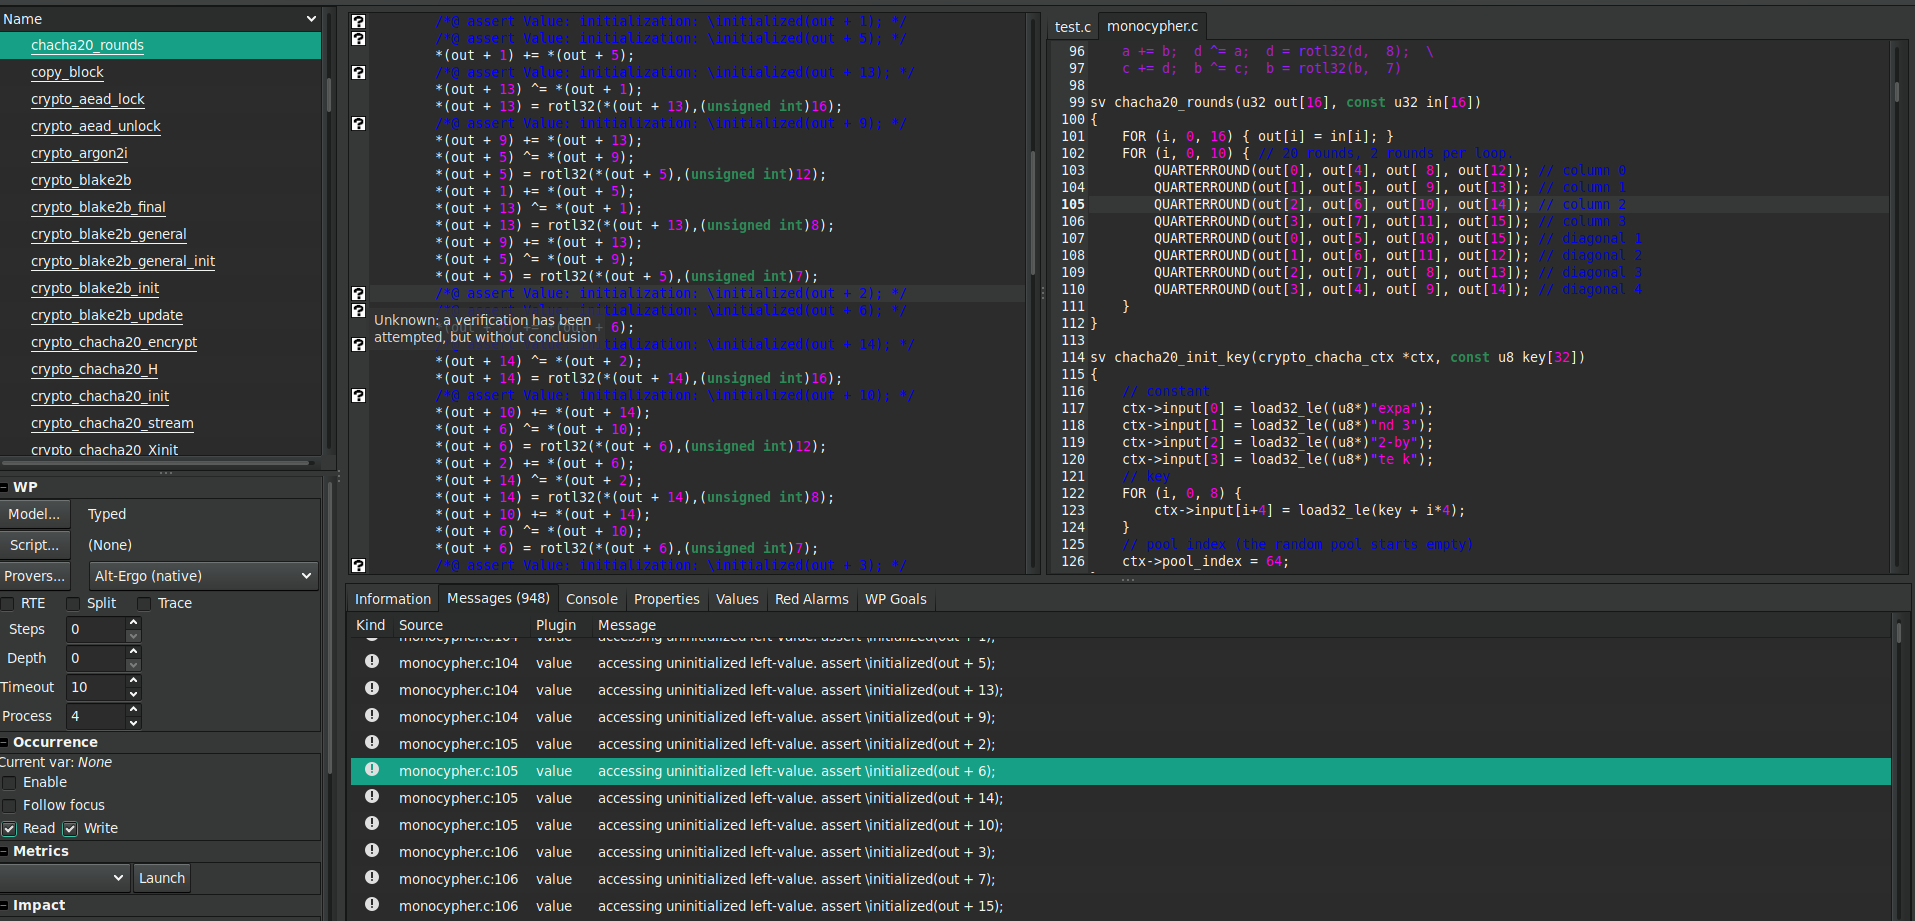
\includegraphics[width=1\textwidth]{img/framagui2}
    \caption{Rezultatele rulării \texttt{Eva}, cu opțiunile de optimizare}
  \label{fig:eva}
\end{figure}

Din analiza capturii de ecran din figura \ref{fig:eva}, constatăm următoarele:
\begin{itemize}
\item avem, în total, 948 de mesaje, vizibile în panoul de jos. Mesajele afișează tipul
  (eroare, alarmă etc.), fișierul sursă care le conține, plugin-ul care a raportat eroarea
  și conținutul mesajului de eroare;
\item click pe un mesaj de eroare deschide exact locul unde s-a raportat eroarea
  și observăm că \texttt{FramaC} a încercat deja să adauge adnotările sugerate;
\item în banda din stînga verificărilor, observăm codificată starea verificării. În imagine,
  se pot vedea multe rezultate de tip $\boxed{?}$, care arată că verificarea nu este
  concludentă: nu se poate spune cu certitudine că în locul respectiv este o eroare sau o
  alarmă falsă.
\end{itemize}

De asemenea, în panoul de jos mai putem vedea și o secțiune în care putem afișa
valorile salvate în diverse variabile.

\begin{figure}[!htbp]
  \centering
    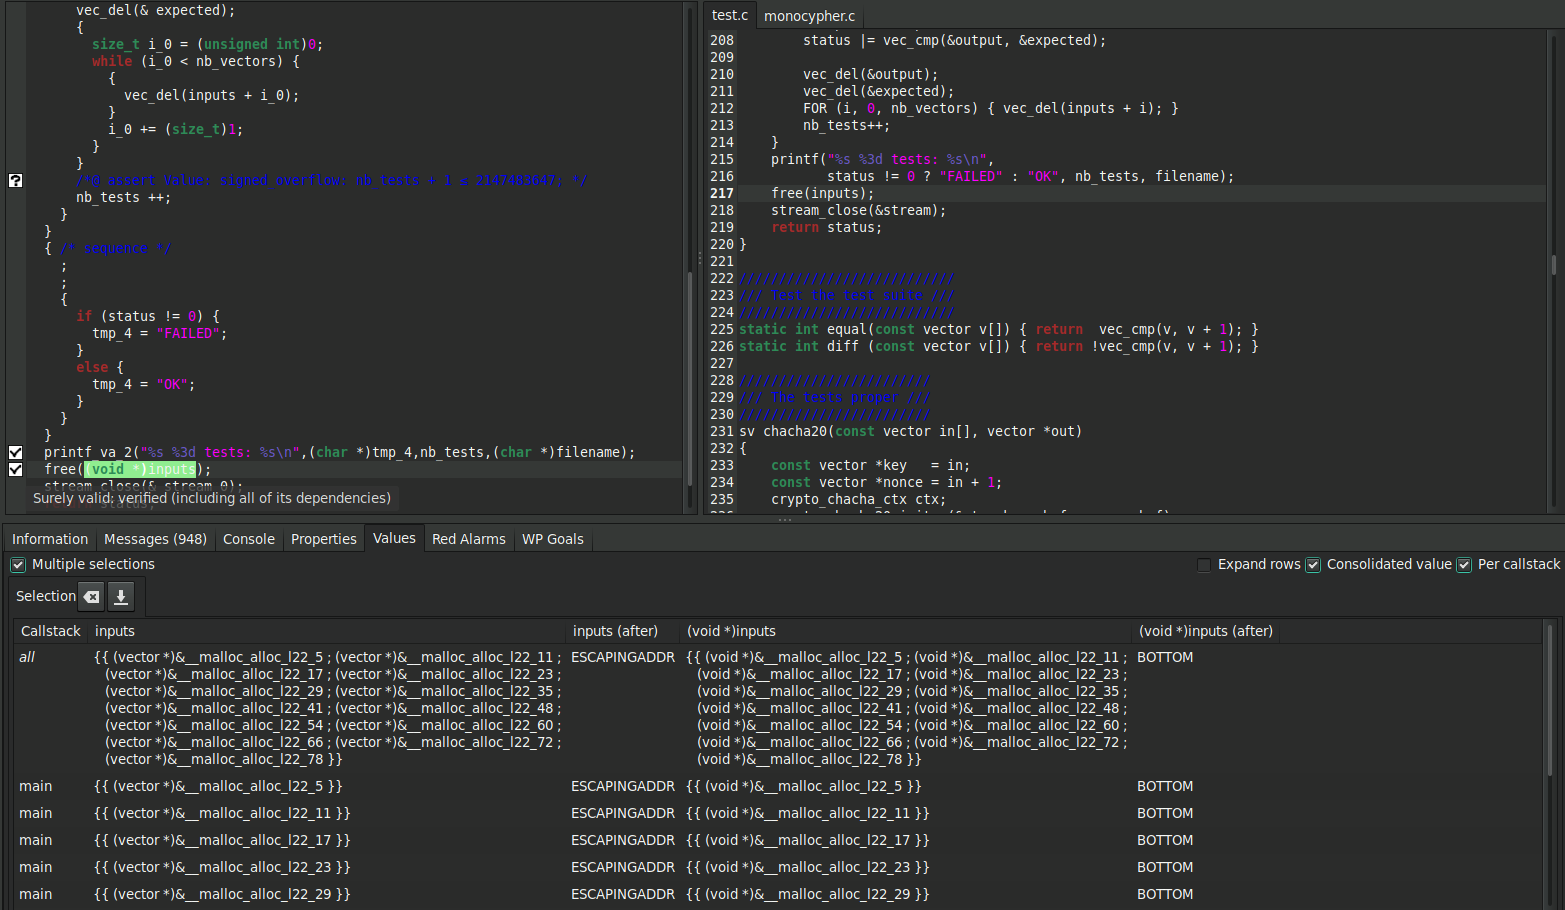
\includegraphics[width=1\textwidth]{img/framagui3}
    \caption{Panoul de valori după verificarea \texttt{Eva}}
  \label{fig:vals}
\end{figure}

În exemplul din figura \ref{fig:vals}, putem să ne concentrăm pe o valoare (\texttt{inputs}) din
\texttt{test.c:217}, în acest caz și, dacă verificăm valorile sale exact înainte și după
apelul funcției \texttt{free}, putem vedea valoarea inițială și cea de după dezalocare
(care devine, desigur, \texttt{BOTTOM}). Totodată, sîntem siguri și că verificarea s-a făcut cu
succes, deoarece în dreptul acestor instrucțiuni, avem semnul bifat, care explicitează în
\texttt{Surely valid.}


%%% Local Variables:
%%% mode: latex
%%% TeX-master: "../mono-frama"
%%% End:
